\chapter{Evaluation}

\section{Customer Requirements}

These are the original objectives specified by the client at the analysis stage of making this system.

\textbf{General Objectives}

\begin{itemize}
	\item To have an interactive and easily navigable graphical user interface, applying a suitable colour scheme and layout
	\item To make the database concise and adjustable
	\item To create various lessons, with a wide range of challenges, which effectively teach students how to do trigonometry and Pythagoras
	\item To create tasks which are relevant to the lessons to be completed by the user in order to test their progress
	\item To allow this progress to be recorded in an easily accessible and readable database
	\item To incorporate algorithms which find and/or check the solution given by the user accurately and give clear and easy to read outputs to correspond with said inputs
	\item To have some access restrictions to certain levels of user
	\item To make the program accessible only from various computers with permissions
\end{itemize}

\textbf{Specific Objectives}

\begin{itemize}
	\item To create a teaching program that uses the new GCSE Maths curriculum, as lots of resources will soon be out of date
	\item To include the following topics: Trigonometry, Pythagoras, 3D Trigonometry, 3D Pythagoras
	\item To include a range of difficulty levels, which can challenge every user's level of ability
	\item Use drag and drop, text boxes and drop down menus for inputs
	\item To include interactive 2D graphics which give a clearer idea of the method being shown to the user
	\item To have a database which can be accessed by different computers online
	\item Use a specific, continuous and attractive colour scheme in every window
	\item To have medium sized, highly visible icons
	\item To have all input buttons randomised to avoid double clicking and guessing from memory
	\item To have small error message windows which pop up and disappear on a timer
	\item To include images and shapes which contrast the colour scheme so they are visible and readable
\end{itemize}

\textbf{Core Objectives}

\begin{itemize}
	\item To create a teaching program that uses the new GCSE Maths curriculum, as lots of resources will soon be out of date
	\item To make the database easy to access and easy to read
	\item To include primarily trigonometry based topics, such as how to use the sine, cosine and tan rules
	\item To include an initial, moderate difficulty in order to cater for a majority of students
	\item To make the database functional and able to store the requested details
\end{itemize}

\textbf{Other Objectives}

\begin{itemize}
	\item To position buttons, text boxes and drag and drop boxes in within the layout of the graphical user interface in such a way that cheating and lucky guessing can be minimised
	\item To make the database adjustable if necessary
	\item Use a more interesting range of input types like drawing boxes rather than just clicking and typing
	\item To include a wider range of difficulties to challenge every student on the right level for them
	\item To include a wider range of topics such as pythagoras, then 3D trigonometry and 3D pythagoras
\end{itemize}

\subsection{Objective: }

To have an interactive and easily navigable graphical user interface, applying a suitable colour scheme and layout

\subsubsection{Objective Met?}

Yes/no 

\subsubsection{Evidence: }

Evidence

\subsection{Objective: }

To make the database concise and adjustable

\subsubsection{Objective Met?}

Yes/no 

\subsubsection{Evidence: }

Evidence

\subsection{Objective: }

To create various lessons, with a wide range of challenges, which effectively teach students how to do trigonometry and Pythagoras

\subsubsection{Objective Met?}

Yes/no 

\subsubsection{Evidence: }

Evidence

\subsection{Objective: }

To create tasks which are relevant to the lessons to be completed by the user in order to test their progress

\subsubsection{Objective Met?}

Yes/no 

\subsubsection{Evidence: }

Evidence

\subsection{Objective: }

To allow this progress to be recorded in an easily accessible and readable database

\subsubsection{Objective Met?}

Yes/no 

\subsubsection{Evidence: }

Evidence

\subsection{Objective: }

To incorporate algorithms which find and/or check the solution given by the user accurately and give clear and easy to read outputs to correspond with said inputs

\subsubsection{Objective Met?}

Yes/no 

\subsubsection{Evidence: }

Evidence

\subsection{Objective: }

To have some access restrictions to certain levels of user

\subsubsection{Objective Met?}

Yes/no 

\subsubsection{Evidence: }

Evidence

\subsection{Objective: }

To make the program accessible only from various computers with permissions

\subsubsection{Objective Met?}

Yes/no 

\subsubsection{Evidence: }

Evidence

\subsection{Objective: }

To create a teaching program that uses the new GCSE Maths curriculum, as lots of resources will soon be out of date

\subsubsection{Objective Met?}

Yes/no 

\subsubsection{Evidence: }

Evidence

\subsection{Objective: }

To include the following topics: Trigonometry, Pythagoras, 3D Trigonometry, 3D Pythagoras

\subsubsection{Objective Met?}

Yes/no 

\subsubsection{Evidence: }

Evidence

\subsection{Objective: }

To include a range of difficulty levels, which can challenge every user's level of ability

\subsubsection{Objective Met?}

Yes/no 

\subsubsection{Evidence: }

Evidence

\subsection{Objective: }

Use drag and drop, text boxes and drop down menus for inputs

\subsubsection{Objective Met?}

Yes/no 

\subsubsection{Evidence: }

Evidence

\subsection{Objective: }

To include interactive 2D graphics which give a clearer idea of the method being shown to the user

\subsubsection{Objective Met?}

Yes/no 

\subsubsection{Evidence: }

Evidence

\subsection{Objective: }

To have a database which can be accessed by different computers online

\subsubsection{Objective Met?}

Yes/no 

\subsubsection{Evidence: }

Evidence

\subsection{Objective: }

Use a specific, continuous and attractive colour scheme in every window

\subsubsection{Objective Met?}

Yes/no 

\subsubsection{Evidence: }

Evidence

\subsection{Objective: }

To have medium sized, highly visible icons

\subsubsection{Objective Met?}

Yes/no 

\subsubsection{Evidence: }

Evidence

\subsection{Objective: }

To have all input buttons randomised to avoid double clicking and guessing from memory

\subsubsection{Objective Met?}

Yes/no 

\subsubsection{Evidence: }

Evidence

\subsection{Objective: }

To have small error message windows which pop up and disappear on a timer

\subsubsection{Objective Met?}

Yes/no 

\subsubsection{Evidence: }

Evidence

\subsection{Objective: }

To include images and shapes which contrast the colour scheme so they are visible and readable

\subsubsection{Objective Met?}

Yes/no 

\subsubsection{Evidence: }

Evidence

\subsection{Objective: }

To create a teaching program that uses the new GCSE Maths curriculum, as lots of resources will soon be out of date

\subsubsection{Objective Met?}

Yes/no 

\subsubsection{Evidence: }

Evidence

\subsection{Objective: }

To make the database easy to access and easy to read

\subsubsection{Objective Met?}

Yes/no 

\subsubsection{Evidence: }

Evidence

\subsection{Objective: }

To include primarily trigonometry based topics, such as how to use the sine, cosine and tan rules

\subsubsection{Objective Met?}

Yes/no 

\subsubsection{Evidence: }

Evidence

\subsection{Objective: }

To include an initial, moderate difficulty in order to cater for a majority of students

\subsubsection{Objective Met?}

Yes/no 

\subsubsection{Evidence: }

Evidence

\subsection{Objective: }

To make the database functional and able to store the requested details

\subsubsection{Objective Met?}

Yes/no 

\subsubsection{Evidence: }

Evidence

\subsection{Objective: }

To position buttons, text boxes and drag and drop boxes in within the layout of the graphical user interface in such a way that cheating and lucky guessing can be minimised

\subsubsection{Objective Met?}

Yes/no 

\subsubsection{Evidence: }

Evidence

\subsection{Objective: }

To make the database adjustable if necessary

\subsubsection{Objective Met?}

Yes/no 

\subsubsection{Evidence: }

Evidence

\subsection{Objective: }

Use a more interesting range of input types like drawing boxes rather than just clicking and typing

\subsubsection{Objective Met?}

Yes/no 

\subsubsection{Evidence: }

Evidence

\subsection{Objective: }

To include a wider range of difficulties to challenge every student on the right level for them

\subsubsection{Objective Met?}

Yes/no 

\subsubsection{Evidence: }

Evidence

\subsection{Objective: }

To include a wider range of topics such as pythagoras, then 3D trigonometry and 3D pythagoras

\subsubsection{Objective Met?}

Yes/no 

\subsubsection{Evidence: }

Evidence
















 
\section{Effectiveness}

%include as many subsections as necessary for your objectives
\subsection{Objective Evaluation}






\section{Learnability}

When I first consulted my client I took into account how much experience they have already had using software such as my system. They are comfortable using the internet, so with the assistance of the user manual they should have no problem installing Python 3.4 and PyQt4. They, along with the other people the client intends to use this system with, have all had experience using similar educational maths programs, such as MyMaths, which have essentially the same purpose as my system. Therefore I tried to make some aspects of the system somewhat similar to the ones conventionally used in educational maths programs, such as the layout, including the navigation of the system, the topics, and the rules of saving and popping error messages, such as making sure all questions have been attempted. None the less, this system would probably be easy enough for less experienced users anyway, as generally the buttons are clearly labelled, appropriately sized, and organised in a convenient way (branch menu). Although some users may have issues finding the exact right topic in the sub-menus, being a reason for the big red return buttons which make it easy to go back and try another menu.

\begin{figure}[H]
	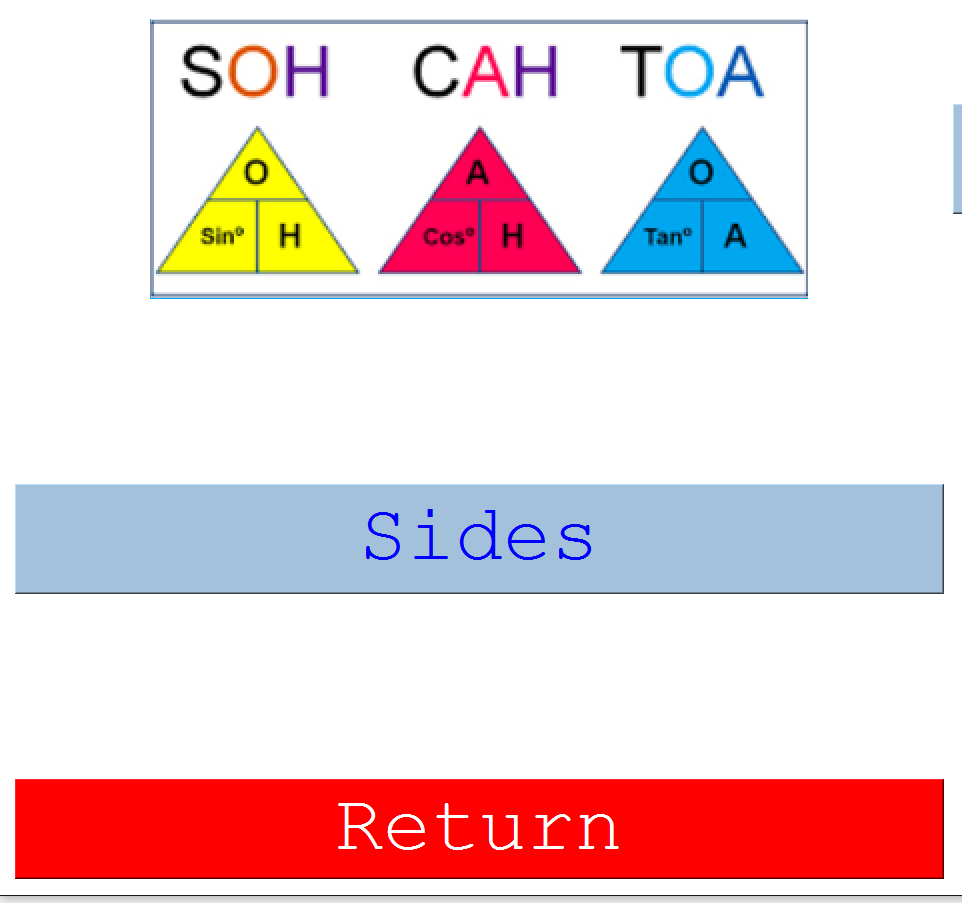
\includegraphics{C:/Users/Jordan/git/COMP4Coursework2/Evaluation/learnability_1}
	\caption{An example of the return buttons used to make navigating the sub-menus easier}
\end{figure}

When designing the system I kept in mind the fact that saving data can be a more complex function if it is done manually, especially by an inexperienced user, so I made all of the database functions automatic; they occur when the user simply clicks a button to finish a homework, or opens the progress screen. This cancels out the need for users to learn new skills which they might not have already learned from using similar systems.

\begin{figure}[H]
	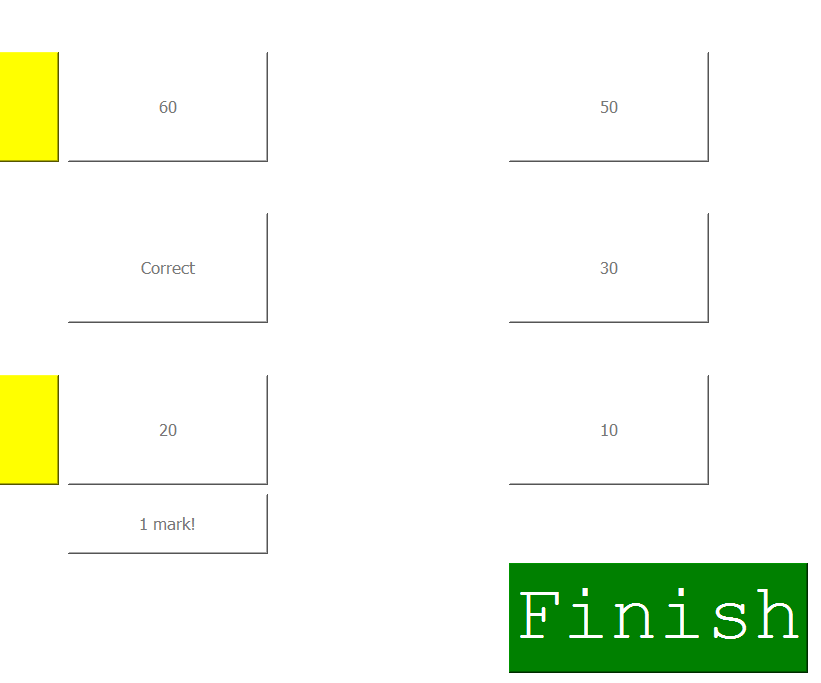
\includegraphics{C:/Users/Jordan/git/COMP4Coursework2/Evaluation/learnability_2}
	\caption{The finish button being clicked to automatically save progress for the user}
\end{figure}

\begin{figure}[H]
	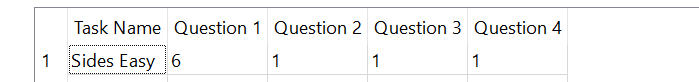
\includegraphics{C:/Users/Jordan/git/COMP4Coursework2/Evaluation/learnability_3}
	\caption{The record which was just saved immediately being updated to the database}
\end{figure}

I also endeavoured to make the database itself very easy to access and understand internally in the system; the system accesses the information from a separate file and displays it in a window in the program, which can be accessed by the user very quickly from the home screen, and even queried for specific details should the user be searching for a specific record. the options in hte combo boxes are as clear as I can make them to make it easier for the user to determine how to use the query function when they try it for the first time.

\begin{figure}[H]
	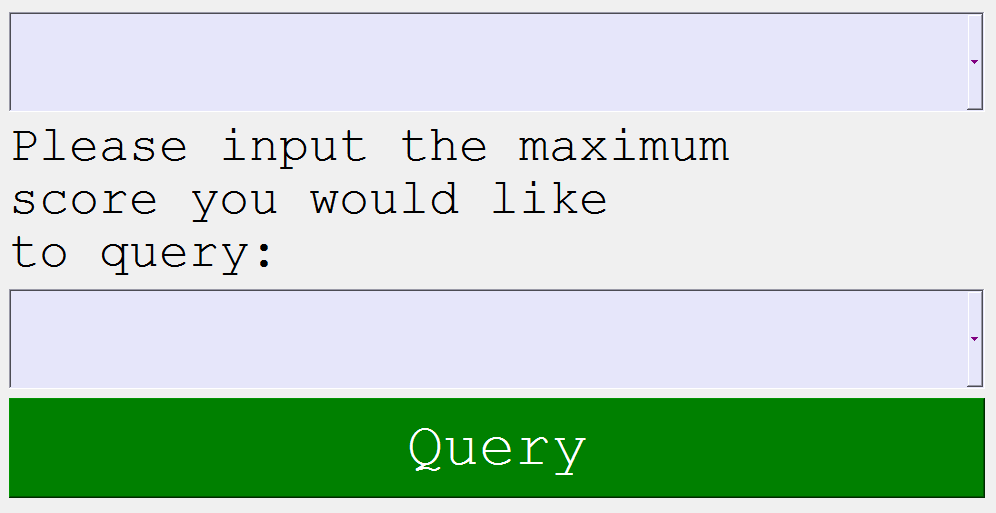
\includegraphics{C:/Users/Jordan/git/COMP4Coursework2/Evaluation/learnability_4}
	\caption{An example of the database being queried for easy access to specific records}
\end{figure}

Error messages were also incorporated to help the user understand why the sytem isn't working as they expected, should they fail to answer a question properly and try to proceed to the next page and be unsure why they cannot.

\begin{figure}[H]
	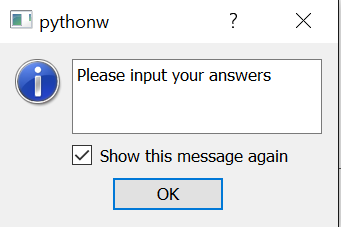
\includegraphics{C:/Users/Jordan/git/COMP4Coursework2/Evaluation/learnability_5}
	\caption{An example of an error message telling the user why they cannot proceed}
\end{figure}

Generally, this system is very easy to use, even for people with little experience with such software, and care has been taken to ensure that the interface is very clear and the error messages are sufficient to help a user fix a progression related problem should they need the help. The only concern is that the user has no way to reset the database internally, so once they start using the system they have to either keep their progress or delete the database file manually.

\section{Usability}

I shall evaluate how easy to use each different aspect of the system is in order to gain an idea of whether or not the overall system has a good level of usability. The criteria I will use to measure the usability of each aspect include readability, convenience, time spent looking across the screen for things and common logic which the user needs to be able to understand.

The graphical user interface has large buttons with clear, blunt text which states the purpose of the button. The buttons also have a user friendly colour scheme which helps to make it clear what might happen when a button is clicked. For example, yellow means to mark an input, blue means to continue to a new screen, and red means to return to a previous screen. This assists the user in distinguishing the purposes of buttons which are sometimes positioned quite close to each other. The sub menus have six buttons, five which open a new menu and one which returns to a past screen, so it helps the user to immediately see which of the six buttons is going to take them back. The user expressed a high level of satisfaction with the user interface in general, suggesting that already it is a very usable interface. All of the input boxes have been sized to match the buttons, and the pictures have been sized to fit in the left over spaces, and to be relevant to the buttons they are placed next to, such as a trigonometry picture next to the trigonometry menu button. The readability of the graphical user interface is good, as all of the text has been enlarged to fill the screen as appropriate, so a user should have no trouble figuring out which buttons to click to find things in the system. The database screen and report widgets are accessible after three mouse clicks, and each lesson or homework after five, so it is convenient to get to any screen if you know where it is. The downside is perhaps having to search through each sub menu to find a topic. All of the widgets are pretty much equally sized, so target acquisition for the users eyes should be fast all round. Finally, each button is labelled appropriately, each picture is relevant and each title is clear, so there is common logic for the user to understand easily when navigating the system. Overall, the graphical user interface has a high usability level.

\begin{figure}[H]
	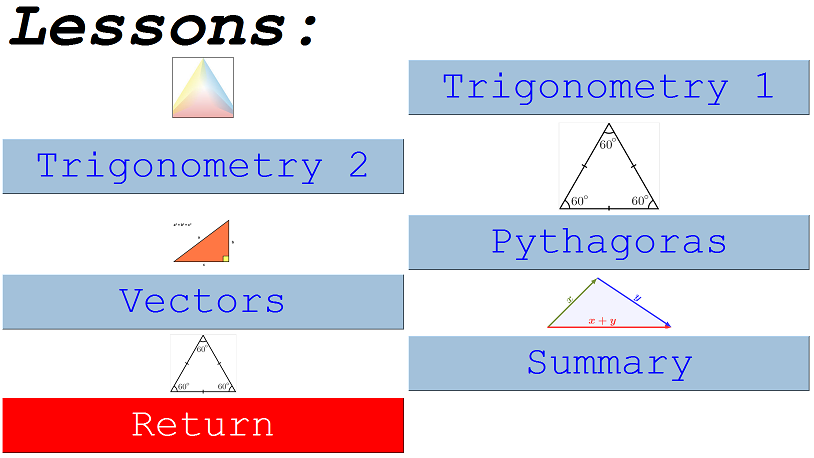
\includegraphics{C:/Users/Jordan/git/COMP4Coursework2/Evaluation/usability_1}
	\caption{An example of the highly readable and easy to navigate menus}
\end{figure}

The storage of data has, in some ways, a high level of usability, but a low level in others. Firstly, it has a high level of usability because the user literally does not have to do any manual saving, loading, or database management, as the system saves and reads everything internally and automatically at certain points. All they need to do is complete the homeworks using easy inputs and maths skills, the learning of which is their responsibility, in order to record progress. They do not need to learn any new skills to be able to maintain the system's records, which can be considered convenient, should the user wish to stick to one 'attempt' at getting the best scores they can from the sytem. However, if the user wanted to delete their current progress and start again, they would have to manually remove the database file in order to reset their progress, which they might not know how to do. the lack of an internal 'drop table' function could be seen as inconvenient, despite it not being the purpose of the system or a client specified objective. Furthermore, the system does not save all of the data which the client wanted to be saved; only about half of the objective information is recorded throughout the system. Therefore the entire database itself has limited usability as the client will struggle to keep track of student's progress as originally intended. The information itself is all displayed in a table widget on the progress screen two clicks away from the welcome screen, so is quick to access and find as it is displayed in a huge table in the top right corner of the screen, one of the places where the user is likely to look first. The text itself is a nice size and is on a well-contraasted white background. In order to improve convenience, time spent and common logic I implemented a report widget where the user can quickly and easily query the database using large and easily usable combo boxes to select query criteria, the results of which will then appear in a similar table widget for the user to view immediately. Overall, the level of usability of the database is moderate, as information can be easily and quickly viewed, and recorded without any extra skills from the user, however once they start using the system they have to stick with the database they have unless they manually delete it.

\begin{figure}[H]
	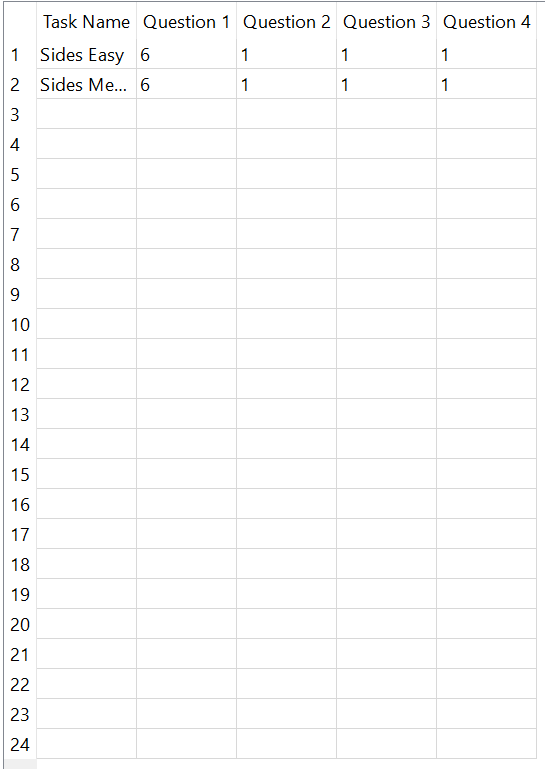
\includegraphics{C:/Users/Jordan/git/COMP4Coursework2/Evaluation/usability_2}
	\caption{Shows the clearly displayed information from the database}
\end{figure}

The subject material used in this system's lessons and homework sections is built up using large, clear text in a readable font against a nicely contrasting background color, accompanied by relevant pictures which can also show the user a mathematical method graphically, and large, clearly purposed buttons, line edits and combo boxes for a variation of input types. The user should have no trouble understanding what the questions are asking of them, and the lessons are supported by sufficient graphical images and text to give the user a clear example of a mathematical technique used to solve a problem. All of the images have either a good or a reasonable resolution. The buttons make it clear how to proceed or return to a previous screen. The colours used are all kind on the eyes. At no point should the user spend more than twenty seconds navigating from screen A to screen B (e.g. welcome screen to a homework screen) as the menus are all easy to use and understand. Therefore, generally the physical appearance of the system gives it quite a high usability.

\begin{figure}[H]
	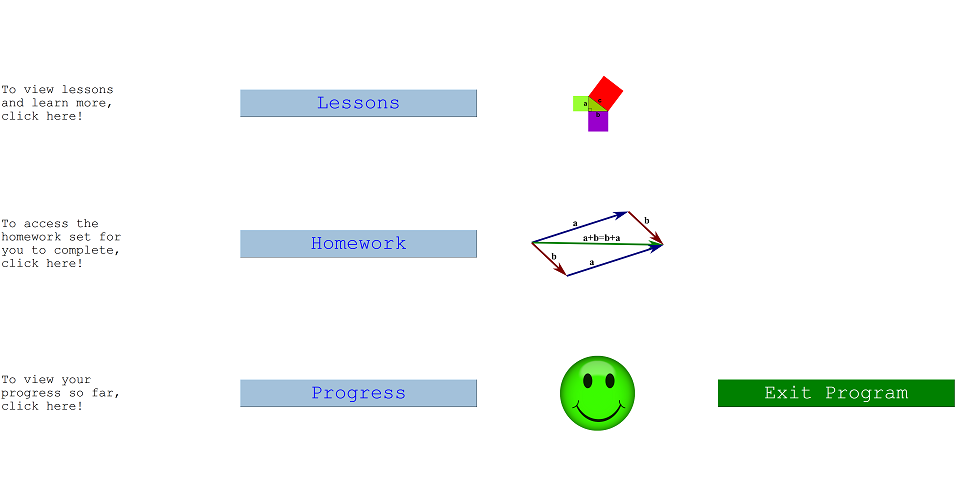
\includegraphics{C:/Users/Jordan/git/COMP4Coursework2/Evaluation/usability_3}
	\caption{The home screen showing the good colour scheme and the high resolution pictures}
\end{figure}

The error messages used in the system have a sole purpose of making it easier for hte user to use, therefore they naturally have a high level of usability. I have ensured that they are easy to understand and dismiss, and only appear when absolutely necessary to minimise disturbance for the user. The only foreseeable potential issue with the error messages is that they are quite small, so the user might have to squint to properly read the text, depending on the size of their monitor and the distance between their eyes and the screen. Otherwise, the text is simple and make it obvious what the problem is (all of the problems which might trigger errors in the system at all are simple ones), and they are dismissable by simply clicking the 'ok' button in the middle. Readibility is limited, convenience is high, as they only appear to help the user, time spent looking is low as they appear right in the middle of the screen making them impossible to miss, and common logic is high as they give clear instructions to the user. Therefore the only thing limiting the error messages' usability slightly is their small size, which is a result of using default QErrorMessage widgets. Otherwise error message usability is overall a high level.

\begin{figure}[H]
	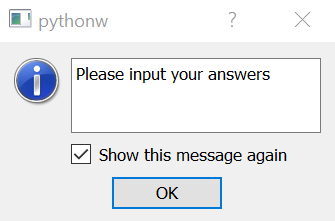
\includegraphics{C:/Users/Jordan/git/COMP4Coursework2/Evaluation/usability_4}
	\caption{An example of the small but clear error messages}
\end{figure}

Conclusively, the usability level of the overall system is reasonably high, as three of the four aspects of the system have been measured to have a high level of usability, and only one has a low-level of usability.

\section{Maintainability}

\section{Suggestions for Improvement}



















\section{End User Evidence}

The following images are of a feedback form which I provided to the client so they could convey to me the extent to which they were satisfied with the system.

\begin{figure}[H]
	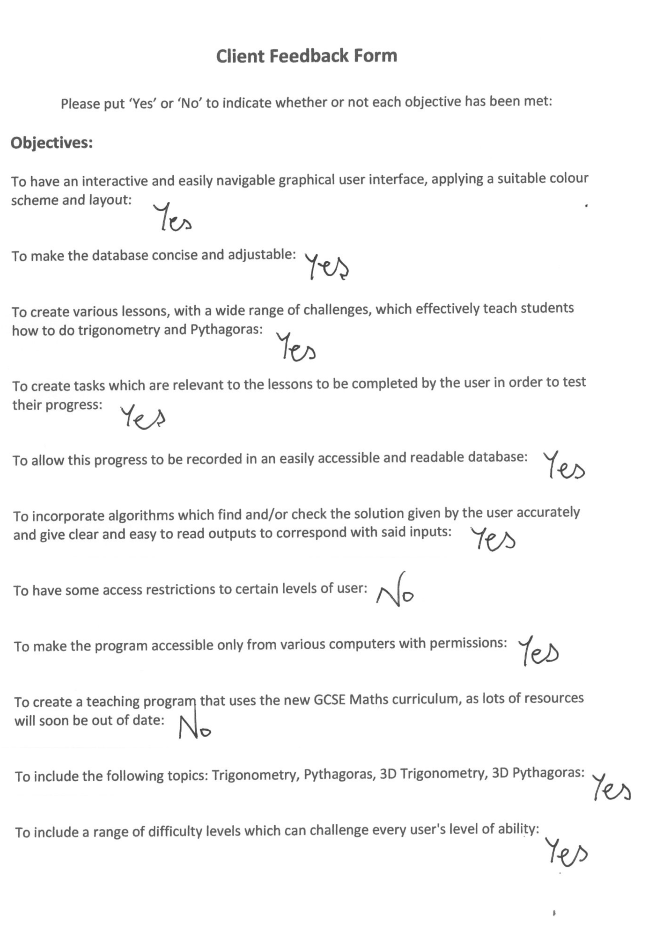
\includegraphics{C:/Users/Jordan/git/COMP4Coursework2/Evaluation/client_feedback_1}
\end{figure}

\begin{figure}[H]
	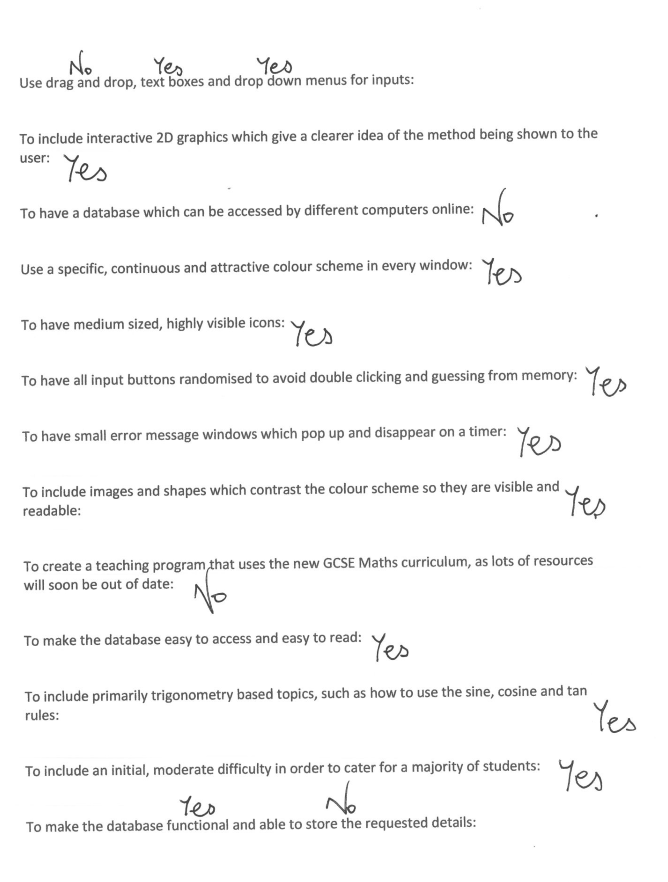
\includegraphics{C:/Users/Jordan/git/COMP4Coursework2/Evaluation/client_feedback_2}
\end{figure}

\begin{figure}[H]
	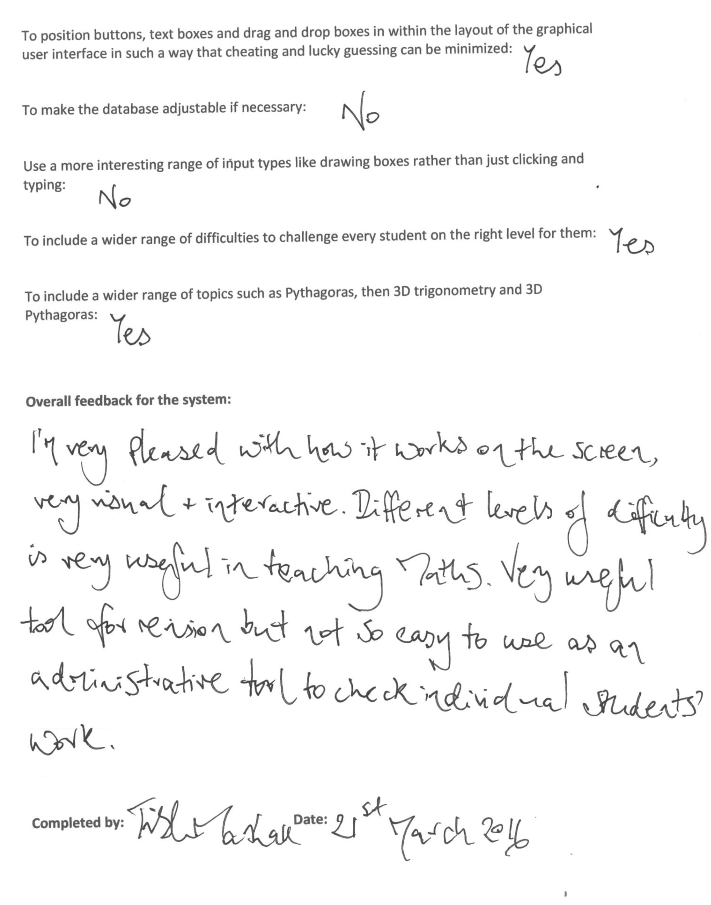
\includegraphics{C:/Users/Jordan/git/COMP4Coursework2/Evaluation/client_feedback_3}
\end{figure}

\subsection{Questionnaires}

This was a brief questionnaire given to the client to give a broad idea of how satisfied they are with the system.

\begin{figure}[H]
	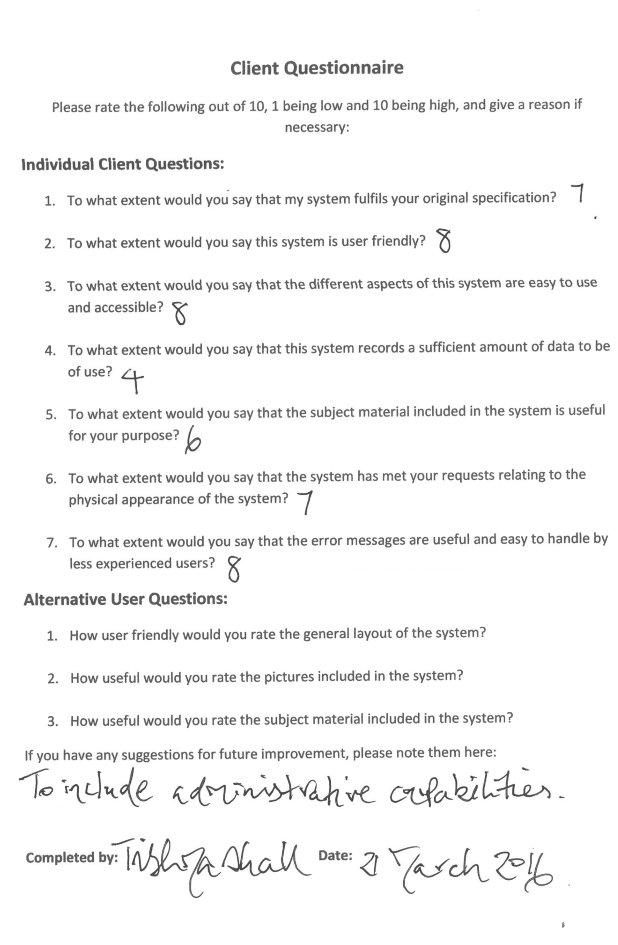
\includegraphics{C:/Users/Jordan/git/COMP4Coursework2/Evaluation/client_questionnaire}
\end{figure}

\subsection{Graphs}

This graph shows the balance of how satisfied the client is with the system:

\begin{figure}[H]
	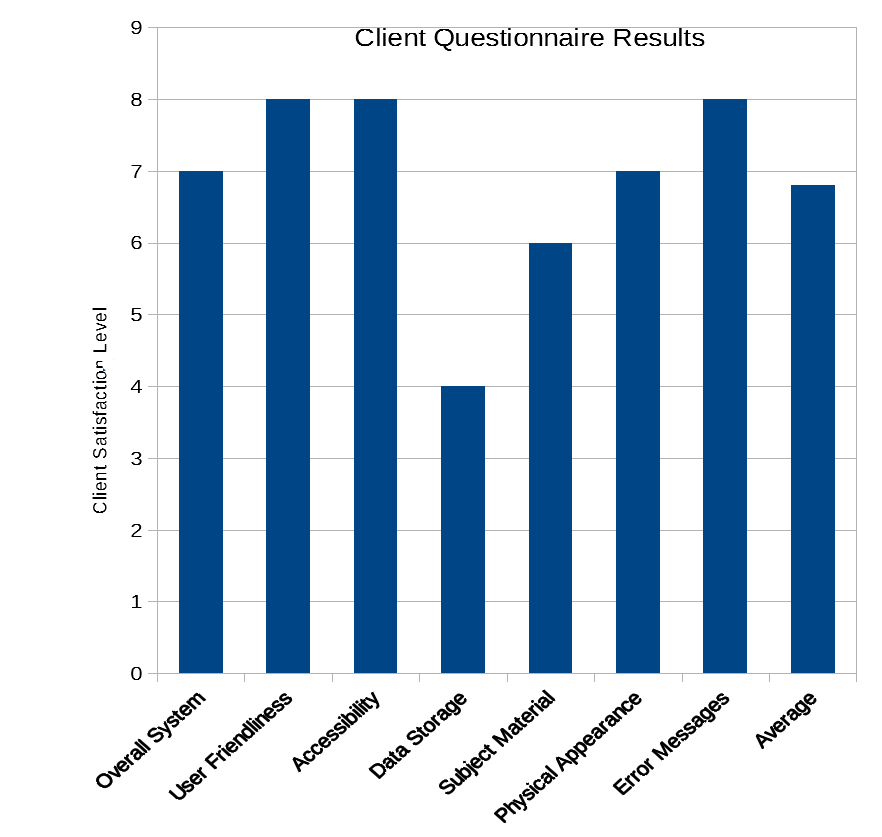
\includegraphics{C:/Users/Jordan/git/COMP4Coursework2/Evaluation/client_graph}
	\caption{According to this graph, the customer was satisfied with 68\% of the system.}
\end{figure}

This graph shows each of the client's 'yes' marks  against the number of 'no' marks related to whether or not each objective was achieved (out of 32 objectives/sub-objectives, some of which were only partially achieved):

\begin{figure}[H]
	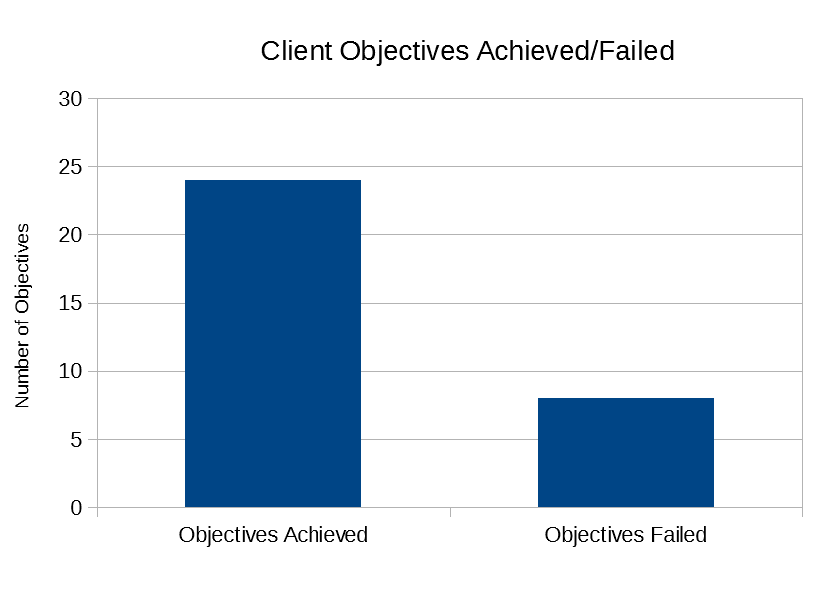
\includegraphics{C:/Users/Jordan/git/COMP4Coursework2/Evaluation/client_graph_2}
	\caption{According to this graph, the customer believed I had achieved 75\% of their specified objectives.}
\end{figure}